%%%%%%%%%%%%%%%%%%%%%%%%%%%%%%%%%%%%%%%%%%%%%%%%%%%%%%%%%%%%%%%%%%%%%%%%%%%%%%%%
%% Plantilla de memoria en LaTeX para la ETSIT - Universidad Rey Juan Carlos
%%
%% Por Gregorio Robles <grex arroba gsyc.urjc.es>
%%     Grupo de Sistemas y Comunicaciones
%%     Escuela Técnica Superior de Ingenieros de Telecomunicación
%%     Universidad Rey Juan Carlos
%% (muchas ideas tomadas de Internet, colegas del GSyC, antiguos alumnos...
%%  etc. Muchas gracias a todos)
%%
%% La última versión de esta plantilla está siempre disponible en:
%%     https://github.com/gregoriorobles/plantilla-memoria
%%
%% Para obtener PDF, ejecuta en la shell:
%%   make
%% (las imágenes deben ir en PNG o JPG)

%%%%%%%%%%%%%%%%%%%%%%%%%%%%%%%%%%%%%%%%%%%%%%%%%%%%%%%%%%%%%%%%%%%%%%%%%%%%%%%%

\documentclass[a4paper, 12pt]{book}
%\usepackage[T1]{fontenc}

\usepackage[a4paper, left=2.5cm, right=2.5cm, top=3cm, bottom=3cm]{geometry}
\usepackage{times}
\usepackage[utf8]{inputenc}
\usepackage[spanish]{babel} % Comenta esta línea si tu memoria es en inglés
\usepackage{url}
%\usepackage[dvipdfm]{graphicx}
\usepackage{graphicx}
\usepackage{float}  %% H para posicionar figuras
\usepackage[nottoc, notlot, notlof, notindex]{tocbibind} %% Opciones de índice
\usepackage{latexsym}  %% Logo LaTeX

\title{Virtual reality editor for virtual reality scenes}
\author{Julian A. Perez Muñoz}

\renewcommand{\baselinestretch}{1.5}  %% Interlineado

\begin{document}

%%%%%%%%%%%%%%%%%%%%%%%%%%%%%%%%%%%%%%%%%%%%%%%%%%%%%%%%%%%%%%%%%%%%%%%%%%%%%%%%
%%%%%%%%%%%%%%%%%%%%%%%%%%%%%%%%%%%%%%%%%%%%%%%%%%%%%%%%%%%%%%%%%%%%%%%%%%%%%%%%
% DISEÑO E IMPLEMENTACIÓN %
%%%%%%%%%%%%%%%%%%%%%%%%%%%%%%%%%%%%%%%%%%%%%%%%%%%%%%%%%%%%%%%%%%%%%%%%%%%%%%%%

\cleardoublepage
\chapter{Resultados}

En esta sección incluiré el manual de usuario de la aplicación donde explicaremos desde un punto de vista del usuario y de  manera sencilla como utilizar la aplicación y la arquitectura en la que se basa el projecto donde explicaremos la estructura y los componenetes usados para la creación de la aplicación.

\section{Manual de usuario} 
\label{sec:manual de usuario}

Existen dos tipos de interacción del usuario con el escenario, según en que modo de escenario se encuentre, modo navegador o mediante el uso de las gafas de realidad virtual.

Si nos centramos en el navegador la forma de interactuar con los elementos de la escena será clickando en ellos, para el movimiento de la camara pulsaremos y arrastraremos con el uso del ratón, para el movimiento del usuario se hará uso de las teclas W, A, S, D.

Por otra parte si usamos la aplicación con las gafas de realidad virtual, la forma de interactuar con los elementos será con los mandos de estas, el momiento de la camara dependerá de donde mire el usuario, para el movimientos usaremos el joystick de uno de los mandos o con el propio movimiento del usuario.

El usuario comeienza frente a la zona de construcción, y al podium. En este apareceran las figuras que vayamos eligiendo en la costrucción de la escena. El menú se enuentra en la parte inferior de la escena junto a tres botones más, el botón que activa la funcinalidad "Modo grupo", el boton que elimina los manejadores y el selector de ambientes.

\begin{figure}[H]
  \centering
  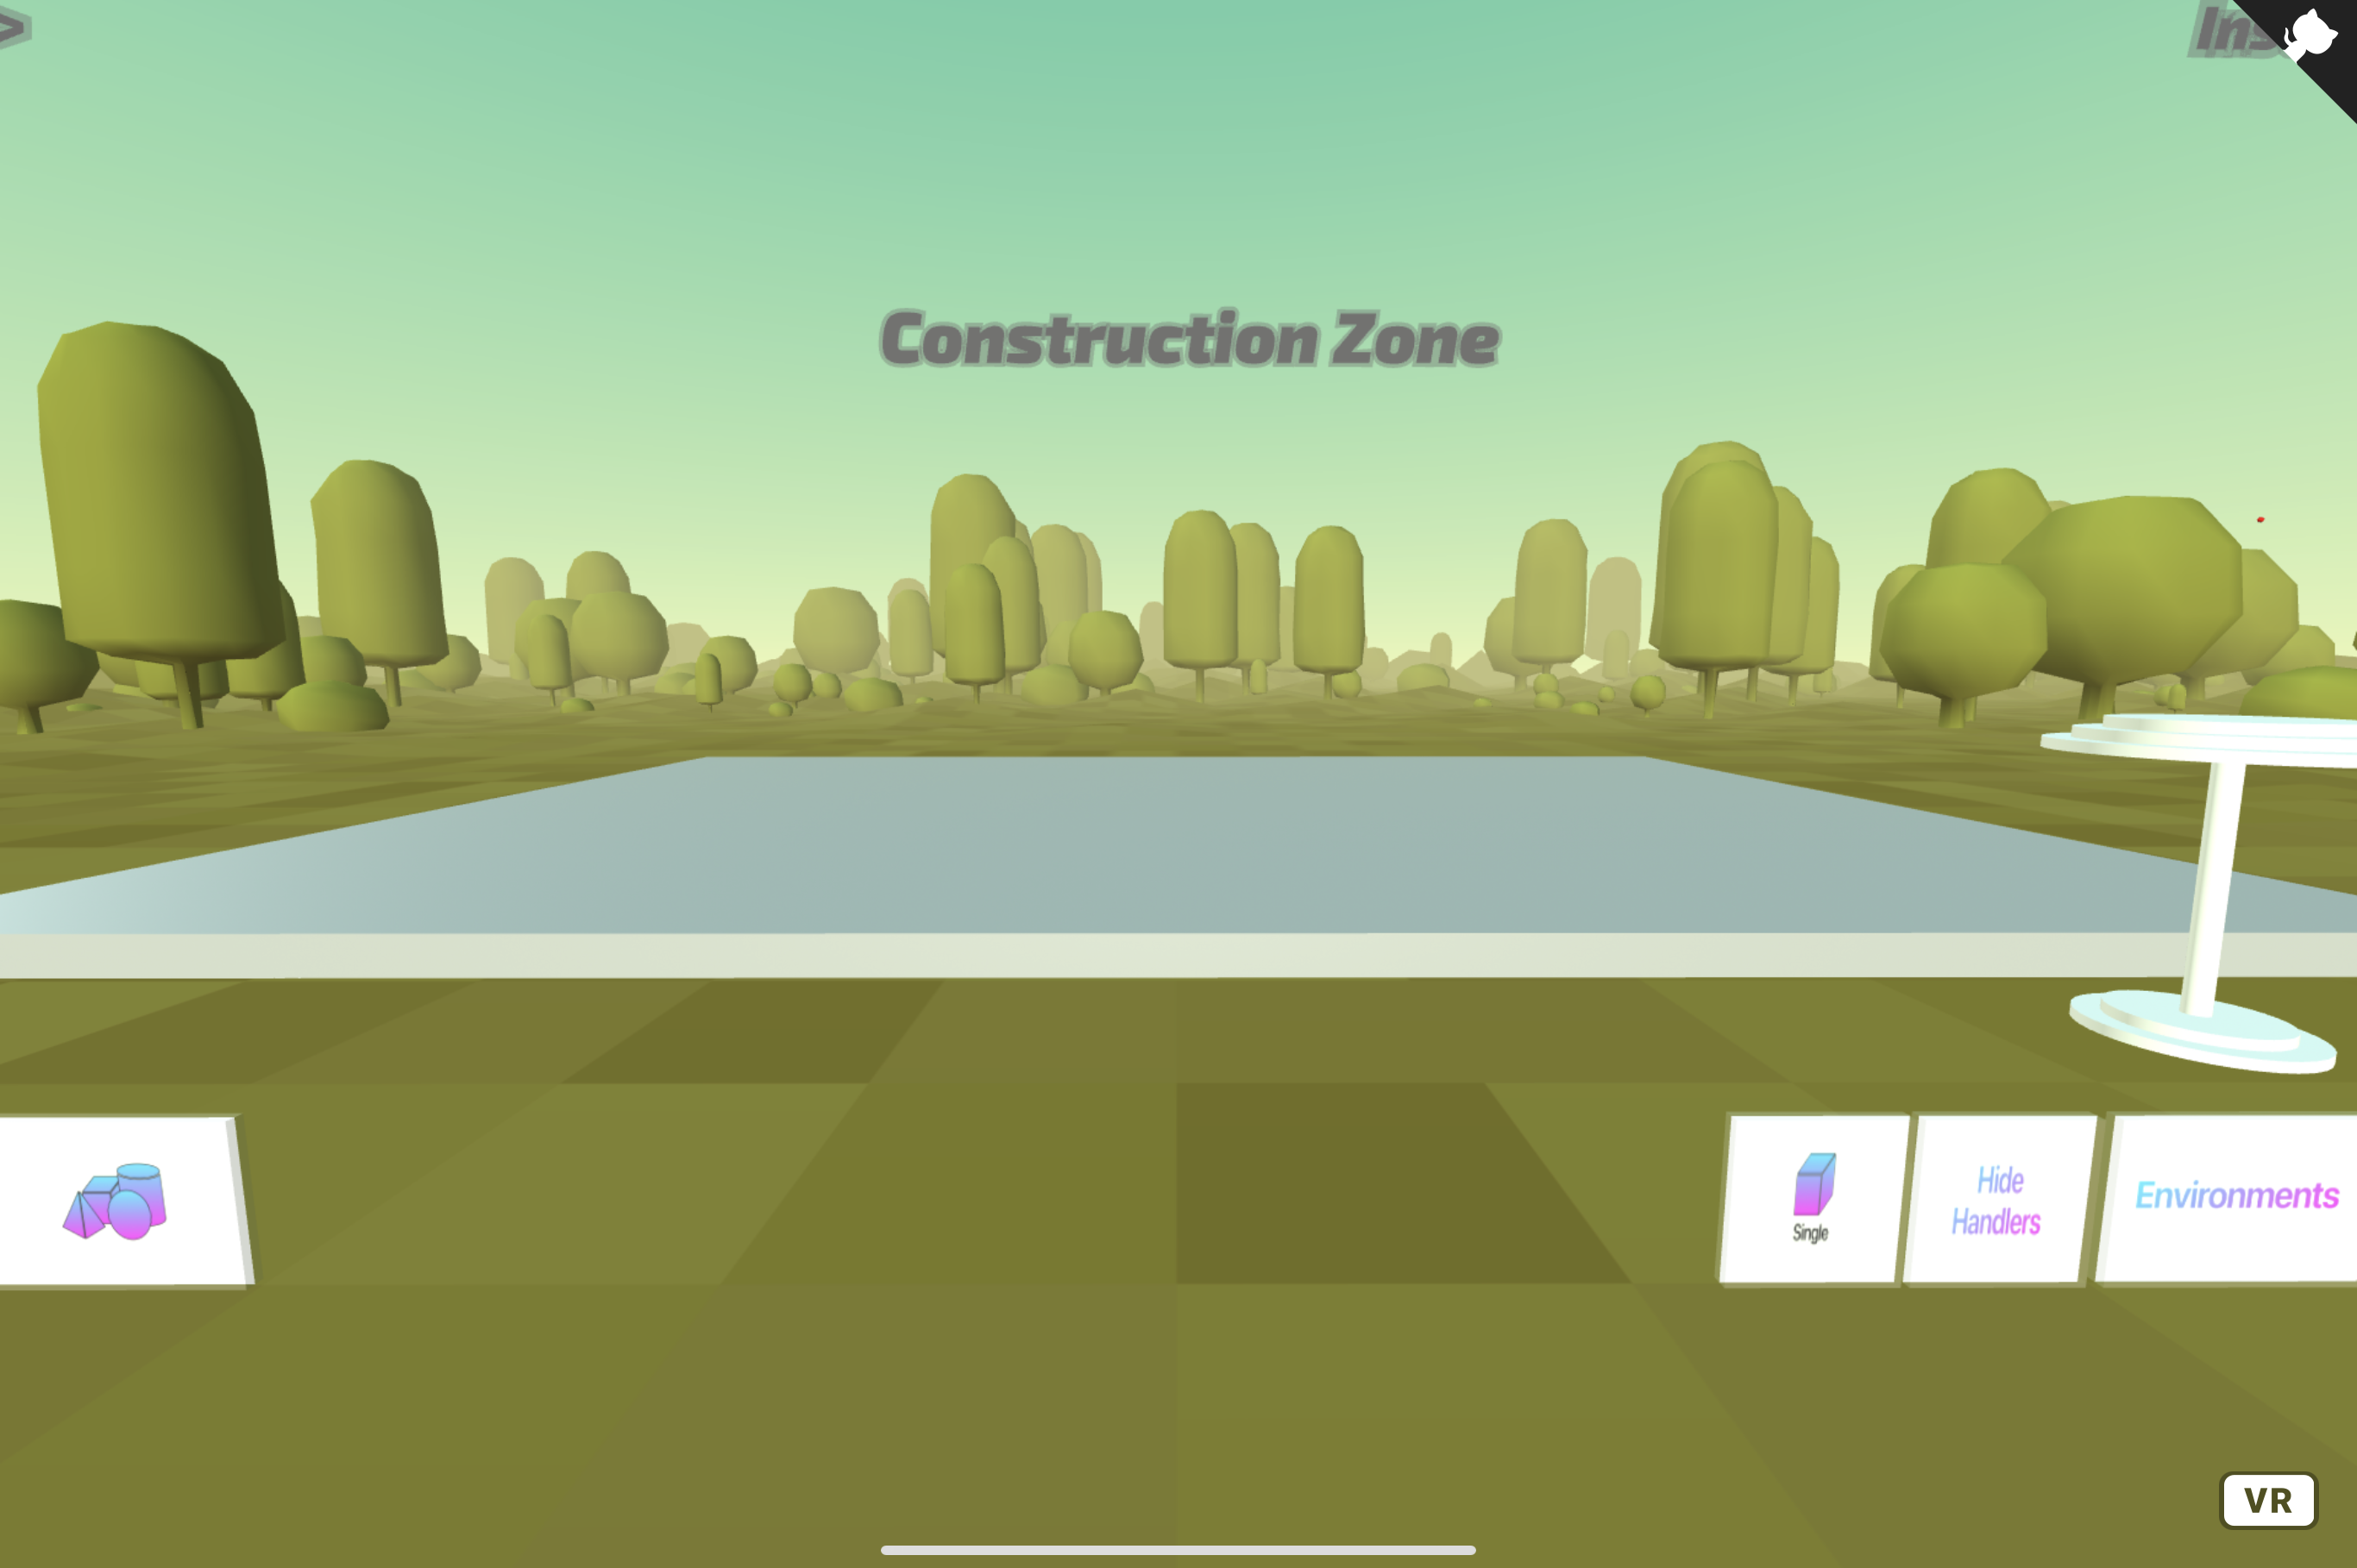
\includegraphics[width=10cm, keepaspectratio]{MemoriaTFG-JulianPerez/img/Editor Scene.png}
  \caption{Inicio página del editor}\label{home}
\end{figure}

Si el usuario pulsa el menú de selector de figuras, podrá elegir tanto las figuras basicas como varios modelos gltfs, si elegimos uno de estos modelos 3D, aparecera un menu en el cual pulsando los botones "+" o "-" podremos modificar dos atributos principales de las figuras, la horientación y el tamaño.

\begin{figure}[H]
  \centering
  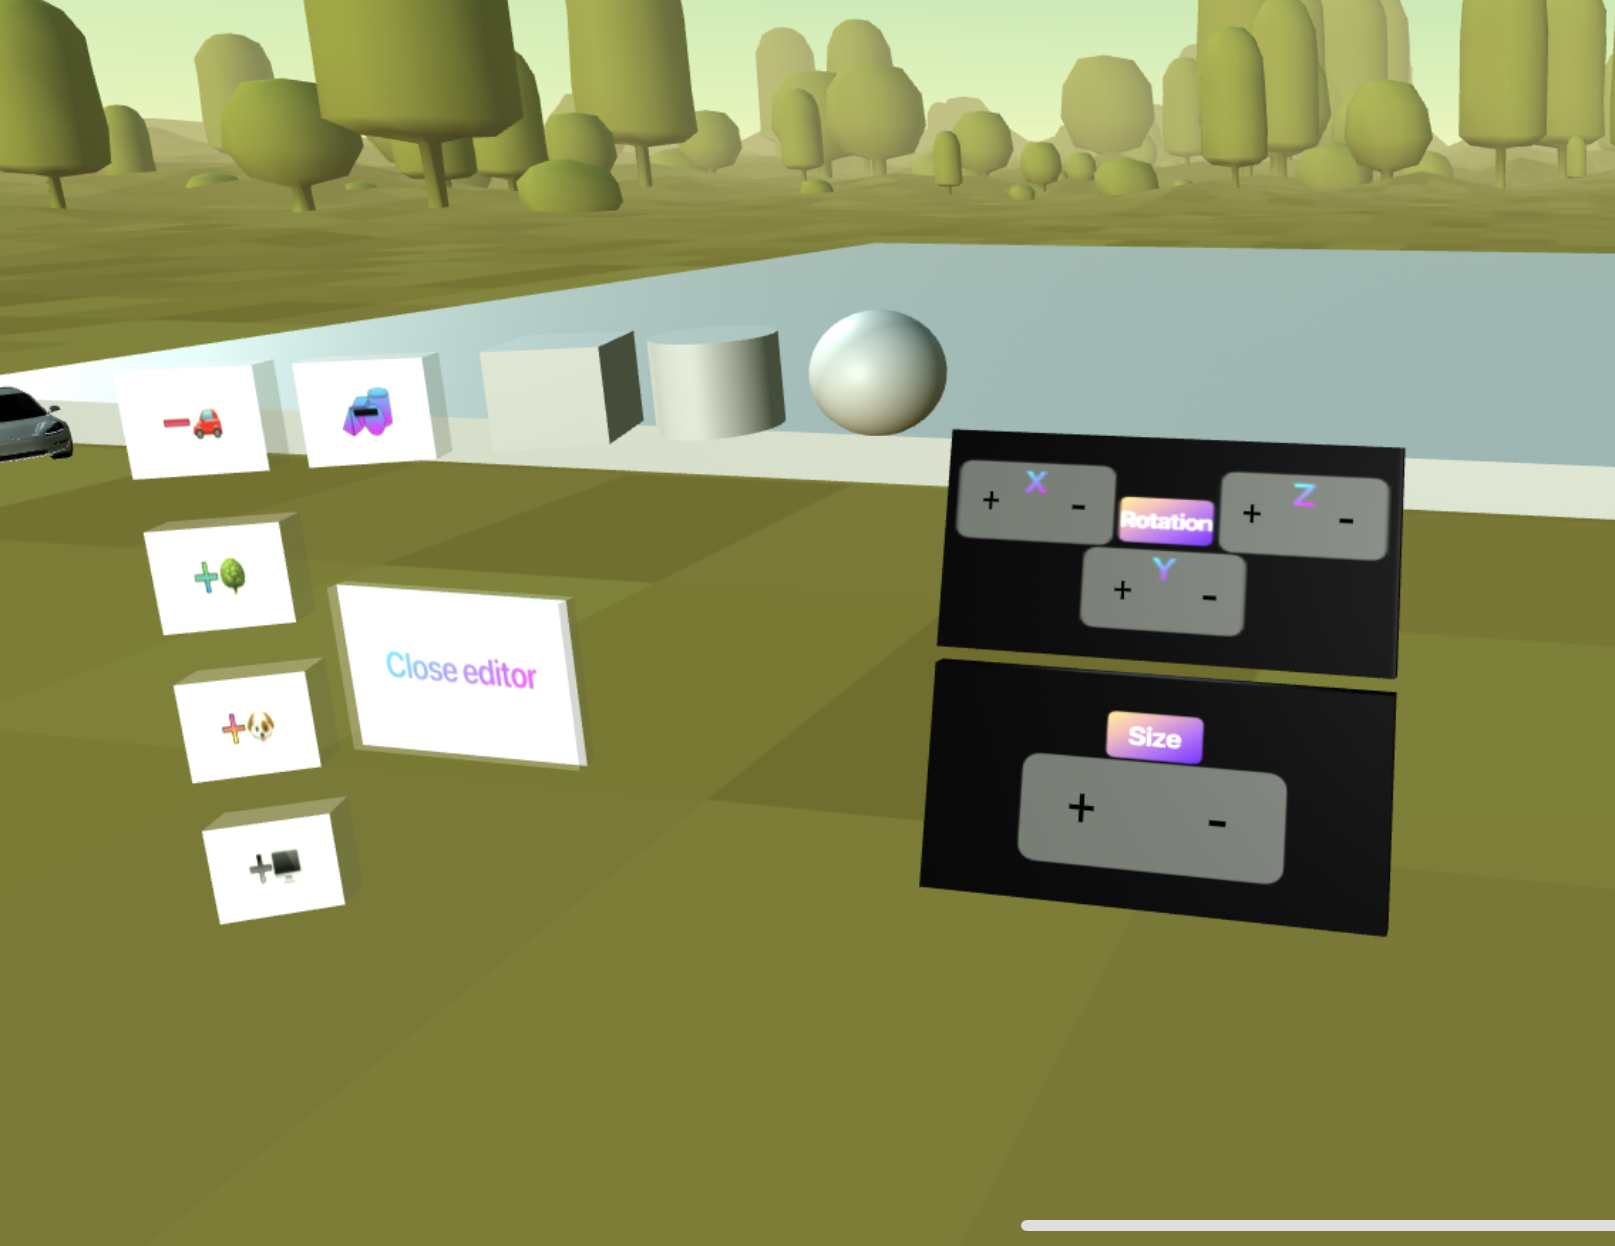
\includegraphics[width=10cm, keepaspectratio]{MemoriaTFG-JulianPerez/img/Screenshot 2021-05-24 at 22.49.26.png}
  \caption{Menú modificación gltfs}\label{home}
\end{figure}

Si por el contrario el usuario pulsa una de las tres figuras básicas, el menú de modificacíon de la figura se aplia de manera notable, podremos modificar del mismo modo que el anterior, pulsando los botones + y -, el tamaño, el color, la horientazión, la transparencia, opacidad, el metalizado y la rugosidad. En la figura 3.16 se puede visualizar dicho menú.

Una vez elegida la figura y las modificaciones correspondientes la cogeremos del podium y la arrastraremos al lugar deseado del escenario. En la figura 3.20 se muestra como se visualiza la figura en el podium.

Para acceder al modo grupo, el usuario pulsará el botón que aparece en la figura 4.3 
\begin{figure}[H]
  \centering
  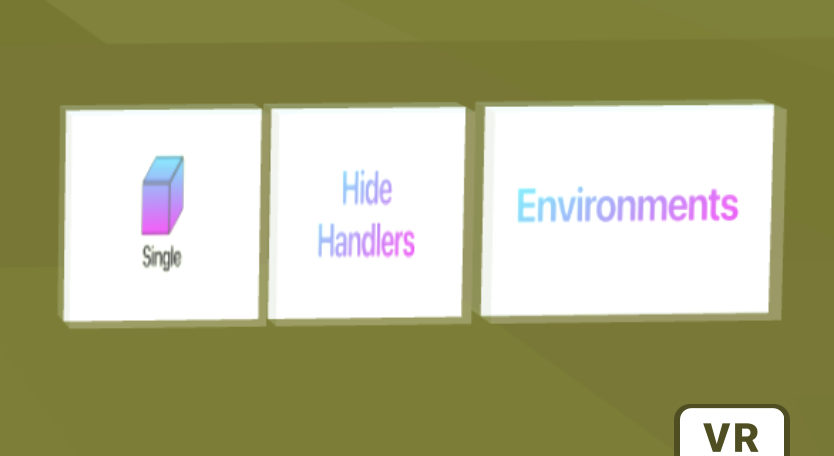
\includegraphics[width=10cm, keepaspectratio]{MemoriaTFG-JulianPerez/img/EditorScene.png}
  \caption{}\label{home}
\end{figure}

Una vez lo pulsemos accedemos al modo grupo, con este activado deberás pulsar las figuras que quieres unir, estas se moveran para hacer ver que son las seleccionadas, una vez ya tengamos todas las figuras seleccionadas deseleccionaremos el modo grupo, crearemos la figura deseada y la moveremos mediante el manejador que se genera en el podium. Mediante la tecla Q se puede activar y desactivar esta funcionalidad y funciona del mismo modo anteriormente explicado.

Si en la escena se visualizan muchos manejadores, estos pueden llegar a molestar, por lo el usuario tiene la posibilidad de ocultarlos pulsando el botón siguiente al modo grupo, 'delete handler'.Como se observa en la figura 4.3

Para cambiar entre distintos ambientes, el usuario tiene la posibilidad de acceder al menu de ambientes que se muestra en la figura 3.24, si pulsamos en él, nos apareceran todos los ambientes que podemos elegir. para poder elegirlos solo tendremos que pulsarlos y el ambiente del escenario cambiará.

Por ultimo en las parte superior tanto izquierda como derecha el usuario se encontrará mediante los cuales poder acceder tanto a la página de inicio como la memoria.

\section{Arquitectura resultante} 
\label{sec:Arquitectura resultante}
En cuanto a la arquitectura de la aplicación, partiremos del esqueleto principal de esta.
\begin{verbatim}
<!DOCTYPE html>
<html>
 <head>
 </head>
<body>

<a-scene id="scn" overlay-visibility>
  <a-assets></a-assets>
  <!-- enviroment-->
  <a-entity id="env" environment="preset:forest"></a-entity>
  <!-- Podium -->
  <a-entity class="podium" podium></a-entity> 
  <!--User Camera-->
  <a-entity>
  <a-box id="showeditor" showeditor></a-box>
  <a-entity id="menu" menu></a-entity>
  <a-entity id="menuenv"></a-entity>
  <a-entity id="editor"></a-entity>
  <a-box id="showhandler" handlereditor></a-box>
  <a-box id="deletehandler" deletehandler></a-box>
  <a-box id="selectenviroments" selectenv></a-box>
  <a-entity gotohome ></a-entity>
  <a-entity gotoinstructiondesktop ></a-entity>
  </a-entity>
</a-scene>
  
 </body>
</html> 
\end{verbatim}

En esta versión simplificada del código podemos ver que este esta separado por diferentes elementos principales en los cuales se iran apoyando los componentes.

Como ya explique anteriormente en el elemento head se introduce todo lo necesario para que a frame y distintos componentes funcionen correctamente.

Dentro del elemeno assets se introducen todas las imagenes, modelos 3D y tambien un elemento llamado mixin que es un plantilla de las figuras básicas para no repetir código en la creación de estas.

Tras el elemento assets, nos encontramos con el elemento que crea el ambiente de la escena y que será modificado dinamicamente mediante un componente que explicaré más adelante.

También nos encontramos con el elemento que crea el podium en el cual generaremos la figuras que vayamos creando.

Por último nos encontramos con el elemento usuario, el cual es padre de otros elementos como son los elementos de los menú de interacción de la escena.

Como ya hemos comentado, cada uno de estos elementos servirán como soporte para los siguientes que se iran creando mediante los componentes que forman el escenario, a continuación pasaré a explicar todos los componentes que  he creado para esta apliación.

Clasificaré los componentes según el elemento al que afecte.


\begin{itemize}
    \item Podium: Este componente se activa al generar el escenario, suvfunción principal es generar la figura de podium mediante la unión de figuras basicas.
\end{itemize}

Los componentes que modifican el comportamiento del selector de figuras son:
\begin{itemize}
    \item showeditor: La activación se realiza pulsando en el bóton del menú de figuras, La funcion de este es, mostras las posibles figuras que puedes crear en el editor, a su vez crea un botón en el cual puedes acceder, mediante el componente que explicare a continuación, a más figuras que poder añadir en la escena.
    \item showmorefigure: Este componente se activa pulsando en el botón que crea el compoente anterior, su función principal es la creación de un menú mediante la creación del componente que explico a continuación  que separa diferentes figuras en diferentes catergorias.
    \item show(vehicles/plants/animals/gadgets): Este componente se activa al pulsar en el menu de categorias que ha creado el componente anterior y su función principal es mostrar nuevos modelos 3d que poder añadir a la escena.

\end{itemize}

Los componentes que modifican los atributos de las figuras que vamos creando son:
\begin{itemize}
    \item editentity: Este componente se activa al pulsar una de las tres figuras principales del editor, crea el menu de modificación de la figura que podemos observar en la figura3.16. Este a su vez crea los componentes que explicare a continuación cuya función son, modificar los atributos de la figura.
    \item changeattribute: Este componente se activa al pulsar en el apartado de cambio de color y su función es cambiar de color a la figura que estemos creando por uno de los disponibles.
    \item (metalness/roughness/opacity)(up/down), Estos componentes se activan al pulsar los botones de + o - en sus respectivos apartados, su función principal como su propio nombre indica es añadir o disminuir, rugosidad, opacidad y metalicidad a la figura.
    \item size(up/down)(x/y/z): Este componente se activa de igual forma que el anterior y se encarga de aumentar o disminuir el tamaño de la figura segun el eje que queramos.
    \item rotation(up/down)(x/y/z) Método de activación similiar a los anterioeres y es el encargado de modificar la rotación de la figura segun el eje que queramos.
    \item dotransparent, Se activa haciendo click en panel que aparece en el menú y  su función principal hacer transparente la figura a crear.
    
    Los dos componentes siguientes no voy a desarrollarlos ya que tienen el mismo comportamiento que los anteriores pero dirigidos a los modelos 3D. La explicación por la que no utilizo los mismos que para las figuras básicas es por que la escala de los modelos 3D es diferente a la de las figuras básicas de A-Frame. En cuanto a la rotación es la misma por lo que utilizamos el mismo componente para todas las figuras. 
    \item editorglts
    \item size(up/down)gltf(x/y/z)
\end{itemize}

    
Sobre la funcionalidad modo grupo podemos distinguir los disitnos componentes:
\begin{itemize}
    \item handlereditor Este componente se activa al pulsar el botón modo grupo que se encuentra en la escena. y se desactiva volviendo a pulsar el botón. Crea un manejador en el podium y mientras esta activado a todos las figuras que clickas, se le añade el componente que explico a continuación.
    \item posibilityofgroup, Este componente se activa al pulsar una figura con el modo grupo activado, se encarga de crear una figura identica a la que hay en el escenario, pero esta vez siendo hija del manejador, de esta manera, cuando lo muevas se moveran también las figuras hijas.
    \item deletehandler Este componente se activa al pulsar el boton delenete handler de la escena, su función es añadir opacidad a todos los manejadores que tenemos en la escena del mismo modo pero al contrario si lo desactivamos.
\end{itemize}

Los componentes que se relacionan con el menú de ambientes son:
\begin{itemize}
    \item selectenv: Este componente se activa pulsando en el menú de selector de ambientes, su función es crear y esconder mas botones en los cuales poder elegir que ambientes, a su vez crea los componentes que paso a explicar a continuación.
    \item env(1/2/3/4/5) Estos componentes se activan cuando pulsas en el botón correspondiente a cada amboente, su función principal es editar el elemento enviroment y cmabiarlo por el elegido.
\end{itemize}

Por ultimo los componentes que añaden comportamiento a los botones para ir a la pantalla de incio y a la de instrucciones son:

\begin{itemize}
    \item gotoeditor(glasses): Se activa al pulsar el texto que te idnica que quieres ir al editor en la patalla de inicio y su funcion es, como su propio nombre indica, ir a la pantalla del editor, como son diferetnes urls tanto la de las gafas como la de versión escritorio se crean dos componentes, en los siguientes componenntes se aplicara del mismo modo.
    \item gotohome(glasses), Este botón esta disponible tanto en la pagina de instrucciones ocmo en la del editor, se activa al pulsar dichos botones y su funcioón es ir a la página de inicio.
    \item gotoinstructions(glasses): Este botón te aparece tanto en la página de inicio como en la página del editor, se activa pulsando en dichos botones y su función es ir a la página de instrucciones
\end{itemize}

Por últmimo cabe desatacar los componentes que nos ofrece A-frame y utilizamos en nuestra aplicación:
\begin{itemize}
    \item clickable: Este componente nos aporta al elemento que lo contiene la cualidad de poder ser clickado para futuros eventos, este componente es utilizando en casi todos nuestros elementos de la aplicación.
    \item grabbable: Este componente nos permite arrastrar a cualquier parte de la escena los elementos que lo contengan. 
\end{itemize}



\end{document}